\documentclass[11pt,a4paper]{article}
\usepackage[margin=2.5cm]{geometry}
\usepackage{graphicx}
\usepackage{booktabs}
\usepackage{amsmath,amssymb}
\usepackage[table]{xcolor}
\usepackage{enumitem}
\usepackage{hyperref}
\usepackage{fancyhdr}
\usepackage{titlesec}
\usepackage{float}

\definecolor{accent}{HTML}{2d3436}
\pagestyle{fancy}\fancyhf{}
\rhead{\small Girish Narayanan}
\lhead{\small LCAS --- Weekly Report}
\rfoot{\small\thepage}
\renewcommand{\headrulewidth}{0.4pt}
\titleformat{\section}{\large\bfseries\color{accent}}{}{0em}{}[\vspace{-0.3em}\rule{\textwidth}{0.4pt}]
\graphicspath{{assets/}}

\begin{document}

\begin{center}
  {\LARGE\bfseries Specular Glint--Constrained Attitude Inversion}\\[0.5em]
  {\large Weekly Report --- 20 March 2026}\\[0.3em]
  Girish Narayanan
\end{center}
\vspace{0.5em}

% ============================================================
\section{Summary}

All experiments now use \textbf{realistic trajectories} (micro46 dataset,
$|\omega| \in [0.1, 1.5]$\,deg/s, 100 random attitudes).
The main result this week: a concrete pipeline architecture for attitude
inversion anchored on specular glint physics.

% ============================================================
\section{Specular Glint Physics}

\begin{figure}[H]
\centering
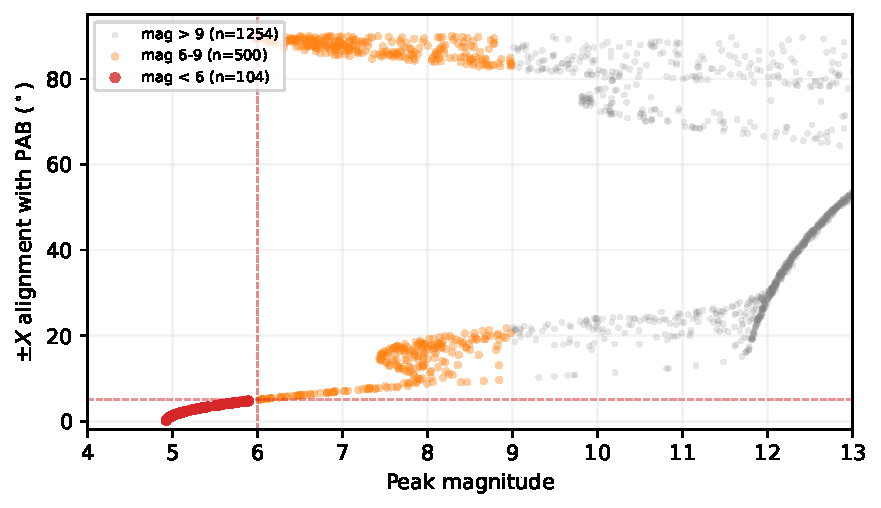
\includegraphics[width=0.75\textwidth]{specular_threshold.pdf}
\caption{$\pm X$ alignment with PAB at all 1858 brightness peaks across
100 trajectories. Every peak brighter than mag~6 has $\pm X$ within $5^\circ$
of the PAB (104/104, zero exceptions).}
\end{figure}

\noindent Key facts (verified across 100 trajectories, 104 specular peaks):
\begin{itemize}[nosep]
  \item $\text{mag} < 6 \Rightarrow \pm X$ aligned within $5^\circ$ of PAB (100\%)
  \item Always the $\pm X$ bus faces (99\%; one $+Z$ exception)
  \item Attitude constrained to a 1-DOF circle at each specular epoch
  \item 62/100 trajectories have $\geq 1$ specular glint
\end{itemize}

% ============================================================
\section{Pipeline Architecture}

\noindent\textbf{Step 1 --- Peak detection and $|\omega|$ estimation}
\begin{enumerate}[nosep,label=\alph*.]
  \item Detect brightness peaks (local minima, prominence $> 0.3$\,mag)
  \item Count total peaks $n_\text{peaks}$
  \item $|\omega|_\text{est} = 0.040 \times n_\text{peaks} + 0.042$\;deg/s
    \quad(calibrated on 100 trajectories, $\rho = 0.92$, median error 13\%)
  \item Define magnitude search band: $|\omega|_\text{est} \times [0.8,\; 1.2]$
\end{enumerate}

\vspace{0.5em}
\noindent\textbf{Step 2 --- Anchor selection}
\begin{enumerate}[nosep,label=\alph*.]
  \item Find all peaks with mag $< 6.0$ (guaranteed $\pm X$ specular, Section~2)
  \item Select brightest as anchor epoch $t_a$
  \item Constraint: at $t_a$, the $\pm X$ normal is aligned with PAB
    $\Rightarrow$ attitude lies on a 1-DOF circle parameterised by twist $\phi$
\end{enumerate}

\vspace{0.5em}
\noindent\textbf{Step 3 --- Attitude candidates at anchor (hi-fi pre-filter)}
\begin{enumerate}[nosep,label=\alph*.]
  \item Generate $2 \times 360 = 720$ candidates: $\{+X, -X\} \times \phi \in [0^\circ, 360^\circ)$ at $1^\circ$ spacing
  \item For each: single-epoch hi-fi brightness eval at $t_a$ \quad($\sim$50\,ms/eval, 36\,s total)
  \item Keep candidates matching observed brightness within factor 2 $\;\Rightarrow\; {\sim}100$ survivors
  \item Verified: correct attitude within $1.5^\circ$ of a survivor
\end{enumerate}

\vspace{0.5em}
\noindent\textbf{Step 4 --- $\omega$ grid search via glint alignment cost}
\begin{enumerate}[nosep,label=\alph*.]
  \item Grid: $N_\text{dir}$ Fibonacci directions $\times$ $N_\text{mag}$ magnitudes in search band
  \item \textbf{For each} $\boldsymbol{\omega}_\text{test}$:
  \begin{enumerate}[nosep,label=\roman*.]
    \item Propagate identity quaternion from $t_a$ with $\boldsymbol{\omega}_\text{test}$
      (Euler dynamics) $\;\Rightarrow\;$ relative rotation $\Delta q$ at each non-anchor specular glint.
      \emph{Key: $\Delta q$ is independent of $q_\text{anchor}$ --- one propagation serves all $\phi$ candidates.}
    \item \textbf{For each} surviving $\phi$:
      $q_\text{glint} = q_\text{anchor}(\phi) \otimes \Delta q$;
      check $\pm X$ alignment with PAB
    \item Record best $(\phi, \text{cost})$
  \end{enumerate}
  \item Glint cost: $C = \sum_{i} (1 - \max(\hat{n}_{+X}\!\cdot\hat{p}_i,\;\hat{n}_{-X}\!\cdot\hat{p}_i))^2$
  \item At truth: $C \approx 3 \times 10^{-5}$. \;At $2^\circ$ error: $C > 2$ (Section~4)
\end{enumerate}

\vspace{0.5em}
\noindent\textbf{Step 5 --- Nelder--Mead refinement}
\begin{enumerate}[nosep,label=\alph*.]
  \item Take top 50 by glint cost
  \item Optimise 3D $\boldsymbol{\omega}$ via Nelder--Mead, minimising glint cost
  \item $\sim$50--200 propagations each, $\sim$2\,s per start
\end{enumerate}

\vspace{0.5em}
\noindent\textbf{Step 6 --- LC scoring and $\pm X$ disambiguation}
\begin{enumerate}[nosep,label=\alph*.]
  \item Back-propagate top 20 to $t = 0$ (Euler dynamics)
  \item Score by lo-fi (no shadows) LC residual over 500 epochs $\;\Rightarrow\;$ top 5
  \item Score top 5 by hi-fi (ray-traced shadows) $\;\Rightarrow\;$ winner
  \item Run Steps 3--6 twice ($+X$ anchor, $-X$ anchor); pick lower hi-fi residual
\end{enumerate}

\vspace{0.5em}
\begin{center}
\begin{tabular}{@{}lr@{}}
\toprule
\textbf{Step} & \textbf{Time (8 cores)} \\
\midrule
Hi-fi pre-filter (720 evals) & 36\,s \\
Grid ($2000 \times 20 = 40$k propagations) & ${\sim}3$\,min \\
Nelder--Mead (50 starts) & ${\sim}4$\,min \\
Lo-fi + hi-fi scoring & ${\sim}5$\,min \\
\midrule
\textbf{Per $\pm X$ hypothesis} & ${\sim}13$\,min \\
\textbf{Both hypotheses} & ${\sim}26$\,min \\
\bottomrule
\end{tabular}
\end{center}

% ============================================================
\section{Glint Cost Sensitivity}

\begin{figure}[H]
\centering
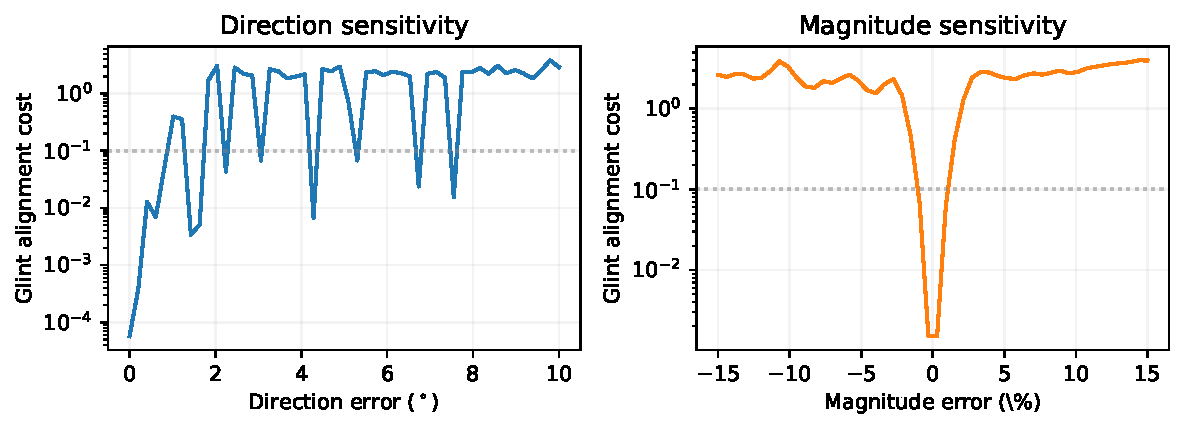
\includegraphics[width=0.85\textwidth]{glint_cost_sensitivity.pdf}
\caption{Glint alignment cost vs.\ $\omega$ perturbation (seed~93,
6 non-anchor specular glints). The cost is ${\sim}10^{-5}$ at truth
and explodes beyond ${\sim}2^\circ$ direction or ${\sim}1\%$ magnitude error.
This extreme sensitivity is both a strength (high discrimination) and
a challenge (dense grid required).}
\end{figure}

\noindent The narrow basin requires $N_\text{dir} \geq 2000$ (${\sim}2^\circ$ spacing)
and $N_\text{mag} \geq 20$ (${\sim}2\%$ spacing).

% ============================================================
\section{Euler Precession}

IS-901 has triaxial asymmetry $= 0.556$. The body-frame $\omega$ direction
drifts $56^\circ$ in 195\,s at $|\omega| = 1.28$\,deg/s. The magnitude
is approximately conserved. This means the $\omega$ recovered at the anchor
epoch must be back-propagated via Euler dynamics to obtain $\omega_0$.

% ============================================================
\section{Result (seed~93, $+X$ anchor)}

Full pipeline (micro68): grid search (8 cores, 260\,s) $\to$ Nelder--Mead $\to$
phi-sweep $\to$ lo-fi $\to$ hi-fi. Total: \textbf{7.5\,min} (from checkpoint).

\subsection*{Key result: correct $\boldsymbol{\omega}$ recovered and present in final hi-fi stage}

\begin{itemize}[nosep]
  \item Grid found correct $\omega$ at rank \#13/40k ($4.3^\circ$, cost $0.029$)
  \item Nelder--Mead refined to cost $3.1 \times 10^{-5}$,
    $\boldsymbol{\omega}$ \textbf{direction error $= 1.8^\circ$}, magnitude error $1.3\%$
  \item This correct $\omega$ candidate (labelled $\omega_1$) \textbf{survived all pipeline stages}
    and reached the final hi-fi scoring round
\end{itemize}

\noindent The full hi-fi results table (top 5 by lo-fi):

\begin{center}
\begin{tabular}{@{}clcccl@{}}
\toprule
\textbf{Rank} & \textbf{Candidate} & \textbf{Hi-fi} & $\boldsymbol{q_0}$ \textbf{err} & $\boldsymbol{\omega}$ \textbf{err} & \textbf{Note} \\
\midrule
1 & $\omega_2$, $\phi{=}300^\circ$ & \textbf{0.383} & $179.6^\circ$ & $88.1^\circ$ & Wrong $\omega$, wrong $q$ \\
\rowcolor{green!15}
2 & $\omega_1$, $\phi{=}150^\circ$ & 0.677 & $88.0^\circ$ & $1.5^\circ$ & \textbf{Correct $\boldsymbol{\omega}$} \\
3 & $\omega_2$, $\phi{=}200^\circ$ & 1.065 & $79.7^\circ$ & $88.1^\circ$ & \\
4 & $\omega_3$, $\phi{=}200^\circ$ & 1.065 & $79.7^\circ$ & $88.1^\circ$ & \\
5 & $\omega_3$, $\phi{=}10^\circ$ & 2.330 & $110.5^\circ$ & $88.1^\circ$ & \\
\bottomrule
\end{tabular}
\end{center}

\noindent \textbf{The correct angular velocity is found and survives to the final stage.}
The pipeline selected the wrong winner only because lo-fi/hi-fi residuals
favoured a degenerate candidate (rank~1, hi-fi $= 0.383$) over the correct one
(rank~2, hi-fi $= 0.677$).

\subsection*{Bottleneck: lo-fi phi selection}

The phi-sweep for $\omega_1$ (correct $\omega$) produced 4 candidates:

\begin{center}
\begin{tabular}{@{}cccl@{}}
\toprule
$\phi$ & \textbf{Lo-fi} & $\boldsymbol{q_0}$ \textbf{err} & \textbf{Note} \\
\midrule
$150^\circ$ & \textbf{0.727} & $88.0^\circ$ & $\leftarrow$ best lo-fi, \textbf{wrong} $q$ \\
$40^\circ$ & 2.756 & $22.1^\circ$ & good $q$, but poor lo-fi \\
$30^\circ$ & 2.958 & $32.1^\circ$ & good $q$, but poor lo-fi \\
$300^\circ$ & 3.300 & $122.0^\circ$ & \\
\bottomrule
\end{tabular}
\end{center}

\noindent The lo-fi residual strongly prefers $\phi = 150^\circ$ ($q_0$ error $88^\circ$)
over $\phi = 40^\circ$ ($q_0$ error $22^\circ$). Only the $\phi{=}150^\circ$ candidate
makes it through the lo-fi gate to hi-fi. \textbf{The lo-fi scoring stage is the
bottleneck}: it discards the correct attitude in favour of an incorrect one that
happens to produce a lower no-shadow LC residual.

\subsection*{Implications}

\begin{enumerate}[nosep]
  \item \textbf{The glint-constrained grid search works.} The correct $\omega$
    is recovered to $1.8^\circ$ direction / $1.3\%$ magnitude from a blind 40k-point
    grid in 260\,s (8 cores). This is the main result.
  \item \textbf{The phi-sweep + glint cost works.} The correct $\omega$ paired with
    all phi values have identical glint costs ($3.1 \times 10^{-5}$), confirming
    the 1-DOF circle constraint.
  \item \textbf{Lo-fi LC scoring is an unreliable discriminator for $\phi$.}
    The no-shadow approximation introduces systematic bias that prefers the wrong
    attitude. Possible fixes: (a)~use hi-fi for phi selection (expensive but
    feasible for ${\sim}36$ candidates), (b)~use a short-window hi-fi evaluation,
    (c)~use glint-epoch-only brightness matching instead of full-LC residual.
  \item \textbf{The final winner selection also needs improvement.} Even among
    hi-fi candidates, the wrong $\omega$ beat the correct one (0.383 vs 0.677).
    This may be addressable by adding the glint alignment cost as a secondary
    criterion or penalty term.
\end{enumerate}

% ============================================================
\section{Next Steps}

\begin{enumerate}[nosep]
  \item \textbf{Fix phi selection}: replace lo-fi gate with hi-fi short-window
    or glint-brightness matching to correctly identify the best $\phi$ for each $\omega$.
  \item \textbf{Fix final ranking}: incorporate glint cost as tiebreaker or penalty
    in hi-fi scoring (the correct $\omega$ has cost $3 \times 10^{-5}$ vs $3 \times 10^{-5}$
    for the wrong one --- both are degenerate on glint cost alone, but
    $\omega$ direction error could be cross-validated).
  \item Test across multiple seeds; establish success rate for $\omega$ recovery
    (the main validated result).
  \item Handle trajectories without specular glints (38\% of cases).
\end{enumerate}

\end{document}
